\documentclass[10pt,twocolumn,letterpaper]{article}

\usepackage[pagenumbers]{cvpr}

\usepackage{microtype}
\usepackage{amsmath}
\usepackage{graphicx}
\usepackage{float}
\usepackage{booktabs}
\usepackage{array}
\usepackage{makecell}
\usepackage{tabularx}
\usepackage{placeins}
\usepackage{siunitx}
\usepackage{ragged2e}
\usepackage{multirow}

\graphicspath{
  {../Content_and_User_Preference_Based_Music_Recommendation_System_Using_Knowledge_Graphs_and_GNN/sec/figures/}
  {../Content_and_User_Preference_Based_Music_Recommendation_System_Using_Knowledge_Graphs_and_GNN/sec/graph_DB/}
  {../Content_and_User_Preference_Based_Music_Recommendation_System_Using_Knowledge_Graphs_and_GNN/sec/kg_plots-2/}
  {../../data/final/}
  {../../data/final/kg_plots/}
}


\definecolor{cvprblue}{rgb}{0.21,0.49,0.74}
\usepackage[pagebackref,breaklinks,colorlinks,allcolors=cvprblue]{hyperref}

\def\paperID{*****}
\def\confName{KG-DL}
\def\confYear{2026}

\title{Milestone Supplement: Training, Experiments, Results, and Contributions}

\author{Group 7 \quad Pedro Fanica (54346) \quad Aarthi Perumpillichira (66404) \quad Maja Skwaroń (66083)}

\begin{document}
\maketitle

% ─────────────────────────────────────────────────────────────────────────────
\section{Training Methods}
\label{sec:training}

\paragraph{Autoencoder.}
A fully connected autoencoder compresses the 1,525-dimensional jSymbolic/music21 feature vector of each track to a 128-dimensional bottleneck via encoder layers $1526\!\to\!512\!\to\!256\!\to\!128$ (symmetric decoder), ReLU + dropout~0.2. Trained with Adam ($lr{=}10^{-3}$, batch 256) to minimise MSE for up to 200 epochs; early stopping triggered if $\Delta{<}10^{-4}$ over 15 epochs.

\paragraph{KGE (RotatE / ComplEx).}
Both models are trained for 100 epochs on 807,955 triples (listening edges excluded). Adam optimiser, entity\_dim=128, batch 32,768, 256 negatives per positive. Output: 256-dimensional vectors for all 304,110 entities.

\paragraph{HGT.}
2 message-passing layers, 4 attention heads, hidden dim 128, dropout 0.1. Track nodes: 384-dim input (128-dim AE $\Vert$ 256-dim RotatE); other types: 256-dim KGE. Per-type MLP head → 64-dim $\ell_2$-normalised output. Trained 200 epochs, Adam ($lr{=}10^{-3}$, wd $10^{-4}$) with cosine-annealing. Checkpoint selected by composite Overall Score at $K{=}10$ on validation.

\textit{Loss}: logit-adjusted listwise cross-entropy with soft engagement targets $\tilde{p}_{ui}\propto\log(1+c_{ui})$:
\begin{equation*}
s_i = \tfrac{\hat{\mathbf{u}}^\top\hat{\mathbf{t}}_i}{\tau} + \lambda\log p_i,\quad
\mathcal{L}=-\tfrac{1}{|B|}\sum_{u,i}\tilde{p}_{ui}\log\mathrm{softmax}(\mathbf{s}_u)_i
\end{equation*}
where $\tau{=}0.1$ and $p_i$ is the Laplace-smoothed marginal listen probability.

\paragraph{KNN-CF.} User--user cosine similarity on the $\ell_2$-normalised interaction matrix; $k{=}6$ neighbours selected by validation sweep.

\paragraph{XGBoost Hybrid.} Top-200 candidates per user retrieved via AE-profile cosine similarity, re-ranked with a gradient-boosted LTR model (\texttt{rank:ndcg@10}, 300 rounds, early stopping 30) on 300-dim feature vectors.

% ─────────────────────────────────────────────────────────────────────────────
\section{Experiments}
\label{sec:experiments}

\begin{itemize}\setlength\itemsep{0pt}
  \item \textbf{Autoencoder compression}: transductive 200-epoch run over 7,013 tracks; MSE monitored per epoch.
  \item \textbf{KGE model comparison}: RotatE vs.\ ComplEx as HGT node initialisers.
  \item \textbf{Init ablation}: full 200-epoch HGT with RotatE-based vs.\ Gaussian random node features.
  \item \textbf{Logit-adjustment ablation}: 30-epoch sweeps over $\lambda\in\{0.0,\allowbreak 0.05,\allowbreak 0.1,\allowbreak 0.2,\allowbreak 0.5\}$.
  \item \textbf{Multi-$K$ evaluation}: all models at $K\in\{5,10,20,50,100\}$; Wilcoxon + Friedman tests on a shared 5,000-user subsample.
\end{itemize}

% ─────────────────────────────────────────────────────────────────────────────
\section{Results and Learning Curves}
\label{sec:results}

\begin{figure}[h]
  \centering
  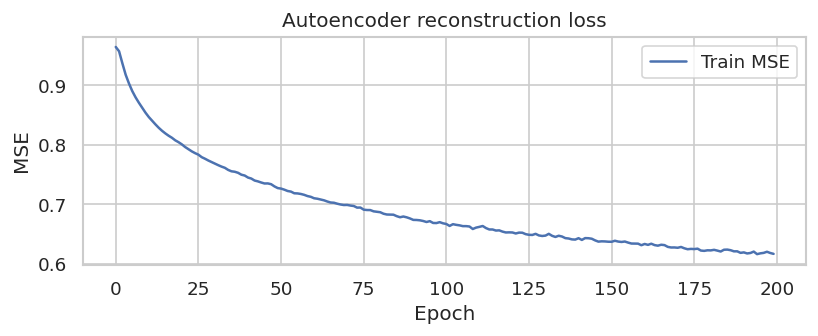
\includegraphics[width=0.92\linewidth]{ae_loss_curve.png}
  \caption{Autoencoder MSE (200 epochs): 0.964 $\to$ 0.616. No early stopping triggered; steepest descent in first 75 epochs. RotatE KGE final loss: 0.356; ComplEx: 0.381 (100 epochs each).}
  \label{fig:ae}
\end{figure}

\begin{table}[h]
\centering\footnotesize
\caption{Test benchmark at $K{=}10$ (all 284,864 test users). Overall $= 0.6\cdot$NDCG $+ 0.2\cdot$Cov $+ 0.2(1-$PB$)$.}
\label{tab:bench}
\setlength{\tabcolsep}{3.5pt}
\renewcommand{\arraystretch}{1.1}
\begin{tabular}{lcccccc}
\toprule
\textbf{Model} & \textbf{Rec.} & \textbf{NDCG} & \textbf{HR} & \textbf{Cov.} & \textbf{PB} & \textbf{Ovrl.}\\
\midrule
MostPopular   & \textbf{.129} & \textbf{.114} & \textbf{.200} & .006 & .611 & .148\\
KNN-CF        & .103 & .106 & .169 & \textbf{.916} & .130 & \textbf{.421}\\
XGBoost       & .038 & .044 & .072 & .667 & \textbf{.118} & .336\\
HGT$^\dagger$ & .001 & .001 & .002 & .046 & .006 & .209\\
\midrule
HGT (self)$^*$& .111 & .071 & --- & .399 & .070 & ---\\
\bottomrule
\multicolumn{7}{l}{\tiny $^\dagger$Directed-eval mismatch (trained undirected, eval directed).}\\
\multicolumn{7}{l}{\tiny $^*$Consistent self-eval (undirected inference, same as training).}
\end{tabular}
\end{table}

\begin{table}[h]
\centering\footnotesize
\caption{HGT ablations at $K{=}10$. Init: RotatE vs.\ random (200 epochs). $\lambda$ sweep (30 epochs).}
\label{tab:abl}
\setlength{\tabcolsep}{3pt}
\renewcommand{\arraystretch}{1.1}
\begin{tabular}{llcccc}
\toprule
& \textbf{Config} & \textbf{Recall} & \textbf{NDCG} & \textbf{Cov} & \textbf{PB}\\
\midrule
\multirow{2}{*}{Init}
  & RotatE & .111 & .071 & .399 & .070\\
  & Random & .118 & .076 & .407 & .069\\
\midrule
\multirow{5}{*}{$\lambda$}
  & 0.00 & .125 & .081 & .006 & .321\\
  & 0.05 & .124 & .079 & .006 & .319\\
  & 0.10 & .118 & .073 & .007 & .305\\
  & 0.20 & .110 & .068 & .015 & .280\\
  & 0.50 & .077 & .048 & .088 & .123\\
\bottomrule
\end{tabular}
\end{table}

KNN-CF achieves the best Overall Score (0.421), dominated by its 91.6\% catalogue coverage. MostPopular leads on per-user NDCG but concentrates recommendations on 0.6\% of the catalogue. Random init marginally outperforms RotatE init for HGT ($\Delta$Recall $+$0.007), suggesting KGE features are subsumed by HGT's own relational learning. The debiasing term $\lambda$ trades ranking quality for coverage: $\lambda{=}0.5$ triples coverage (0.6\%~$\to$~8.8\%) while halving Recall (0.125~$\to$~0.077). All pairwise Wilcoxon and $t$-test comparisons are significant ($p<0.001$).

% ─────────────────────────────────────────────────────────────────────────────
\section{Member Contributions}
\label{sec:contributions}

\begin{description}\setlength\itemsep{2pt}
  \item[\normalfont\textbf{Pedro Fanica (54346)}] Pipeline architecture, \texttt{nb\_env.py} bootstrap, GraphDB upload and SPARQL validation, HGT training loop with logit-adjusted loss, latent-space GMM/UMAP analysis (\S13), cold-start persona GUI (\S14).

  \item[\normalfont\textbf{Aarthi Perumpillichira (66404)}] KG design and construction: OWL ontology schema, \texttt{kg\_builder.py}, Wikidata entity alignment, decade temporal chain, rich KG reification, SPARQL query library and GraphDB inspection.

  \item[\normalfont\textbf{Maja Skwaroń (66083)}] Data processing pipeline: LakhMSDLinker, user taste profile filtering, jSymbolic and music21 feature extraction, symbolic-feature autoencoder, KNN-CF and XGBoost baselines, evaluation protocol and statistical significance tests.
\end{description}

{
  \small
  \bibliographystyle{unsrtnat}
  \bibliography{main}
}

\end{document}
